\documentclass[12pt,letterpaper]{article}
\usepackage[utf8]{inputenc}
\usepackage[spanish]{babel}
\usepackage{amsmath}
\usepackage{amsfonts}
\usepackage{amssymb}
\usepackage{graphicx}
\title{Tarea 3 \\ Optimizacion de Flujo de Redes}
\author{L. A. Gutierrez}
\begin{document}
\maketitle

\section*{Introduccion}
En esta practica se implementaron los algoritmos Ford-Fulkerson y Floyd-Warshall y se midieron los tiempos de ejecucion en instancias de N tamaño empezando en 100 nodos e incrementando de 200 en 200 hasta 2500 nodos. 
Utilicé el codigo fuente del curso de Matemáticas discretas.\footnote{ https://elisa.dyndns-web.com/teaching/mat/discretas/md.html }

\section*{Ford-Fulkerson y Floyd-Warshall}
El FF(Ford-Fulkerson)\footnote{ \label{1} https://reynolds09.wordpress.com/2012/03/26/algoritmo-de-ford-fulkerson/ }
 es un algoritmo para encontrar el flujo máximo de un grafo.
\\ La complejidad teórica del Ford-Fulkerson es $O(qn)$ siendo $q$ la cantidad de Aristas y $n$ la cantidad de nodos$^{\ref{1}}$.

El FW(Floyd-Warshall)\footnote{ https://www.ecured.cu/Floyd-Warshall} 
 es un algoritmo para encontrar el flujo mínimo de un grafo ponderado.

\section*{Medición}
Para medir el tiempo se uso el comando \textit{time} antes de la ejecución de cada programa en \textit{python} en la terminal de ubuntu.

	\textbf{Ej: \textit{time python3 main.py}}

Se realizaron las mediciones con todas las aplicaciones cerradas, solo la terminal funcionando, para obterner una muestra limpia.

Se ejecutó el programa 5 veces, las cuales fueron para hacer una media de la duracion con la misma cantidad de nodos, asi como el máximo y mínimo tiempo de ejecucion, como valores necesarios para poder graficar nuestros tiempos de ejecución.

Todos los tiempos de ejecución se tomaron a mano y luego se transcribieron en una hoja de cálculo que sirvio para el preprocesamiento de los datos antes de graficar.

\section*{Resultados}
Los resultados se muestran en la siguiente grafica.\\
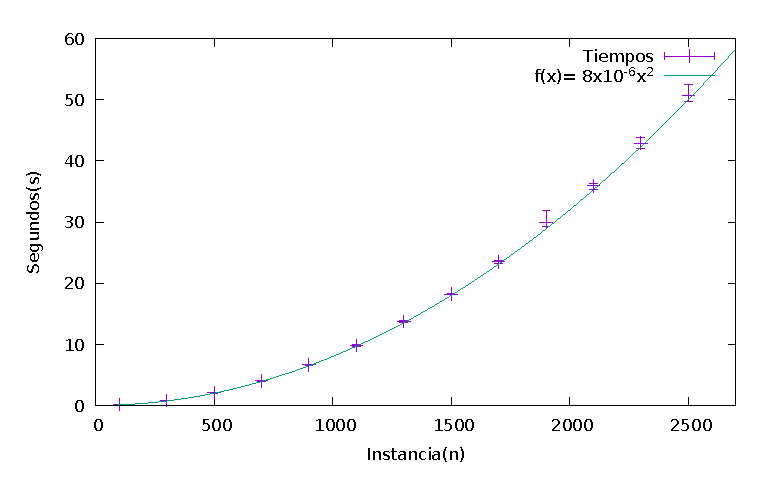
\includegraphics[scale=1]{tiempos} 


En esta ocasión los resultados quedaron en una recta que, por metodos de prueba y error, obtuvo una aproximacion a $8x10^{-6}x^2$ (recta en color verde).



\end{document}